\documentclass[tikz,border=2pt]{standalone}
\usepackage{amsmath,amssymb}
\usepackage{tikz}
\usetikzlibrary{matrix}

\begin{document}
% Upper triangular: everything below the main diagonal is zero; the determinant is the product
% of the diagonal and the diagonal entries are the eigenvalues.
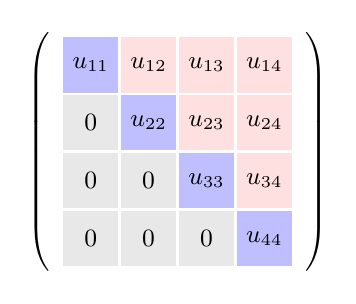
\begin{tikzpicture}[every node/.style={font=\small}]
	\matrix (U) [matrix of math nodes, nodes={minimum size=7mm, anchor=center}, left delimiter=(, right delimiter=), column sep=1pt, row sep=1pt] at (0,0) {
		|[fill=blue!25]| u_{11} & |[fill=red!12]| u_{12} & |[fill=red!12]| u_{13} & |[fill=red!12]| u_{14} \\
		|[fill=gray!18]| 0 & |[fill=blue!25]| u_{22} & |[fill=red!12]| u_{23} & |[fill=red!12]| u_{24} \\
		|[fill=gray!18]| 0 & |[fill=gray!18]| 0 & |[fill=blue!25]| u_{33} & |[fill=red!12]| u_{34} \\
		|[fill=gray!18]| 0 & |[fill=gray!18]| 0 & |[fill=gray!18]| 0 & |[fill=blue!25]| u_{44} \\
	};
\end{tikzpicture}
\end{document}
